%%%%%%%%%%%%%%%%%%%%%%%%%%%%%%%%%%%%%%%%%%%%%%%%%%%%%%%%%%%%%%%%%%%%%%%%%%%%%%%%%%%%
% Document data
%%%%%%%%%%%%%%%%%%%%%%%%%%%%%%%%%%%%%%%%%%%%%%%%%%%%%%%%%%%%%%%%%%%%%%%%%%%%%%%%%%%%
\documentclass[12pt]{article} %report allows for chapters
%%%%%%%%%%%%%%%%%%%%%%%%%%%%%%%%%%%%%%%%%%%%%%%%%%%%%%%%%%%%%%%%%%%%%%%%%%%%%%%%%%%%
\usepackage{preamble}

\begin{document}

\begin{center}
   \textsc{\large MATH 272, Homework 1, \emph{Solutions}}\\
\end{center}
\vspace{.5cm}

\begin{problem}
Plot the following curves and print pictures of each using GeoGebra.  
\begin{enumerate}[(a)]
	\item (Helix) $\curvegamma_1(t) = \begin{pmatrix} 3\cos(t) \\ 3\sin(t) \\ t\end{pmatrix}$, from $t=0$ to $t=2\pi$. Where might this show up? If you think about the Earth moving through space and Moon orbiting Earth, then the Moon follows a (locally) helical path.
	
	\item (Falling Ball) $\curvegamma_2(t) = \begin{pmatrix} t\\  0.5t \\ 9-t^2 \end{pmatrix}$ from $t=0$ to $t=3$.
	
	\item (Trefoil knot) $\curvegamma_3(t) = \begin{pmatrix} \sin(t)+2\sin(2t) \\ \cos(t)-2\cos(2t) \\ -\sin(3t) \end{pmatrix}$ from $t=0$ to $t=2\pi$. (Note that this is the simplest nontrivial \emph{knot}. See: \url{https://en.wikipedia.org/wiki/Trefoil_knot} to learn more.)
	
	\item Create your own curve.
\end{enumerate}
\end{problem}

\begin{solution}~
\begin{enumerate}[(a)]
    \item Here is the plot.
    \begin{figure}[H]
        \centering
        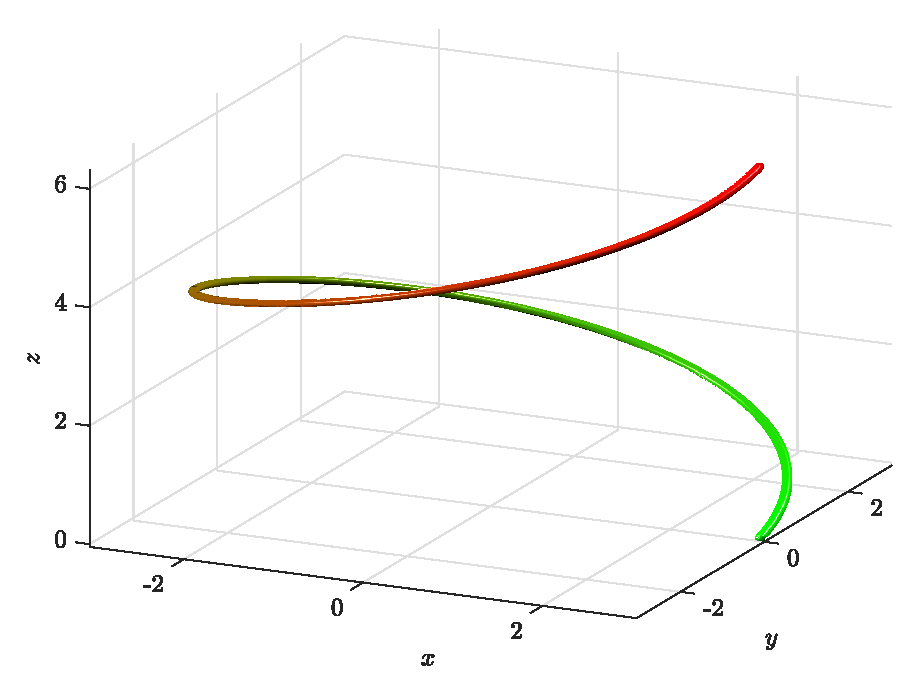
\includegraphics[width=.65\textwidth]{figures/helix}
        \caption{Helical curve. $t=0$ bright green and $t=2\pi$ red.}
    \end{figure}
    \item Here is the plot.
    \begin{figure}[H]
        \centering
        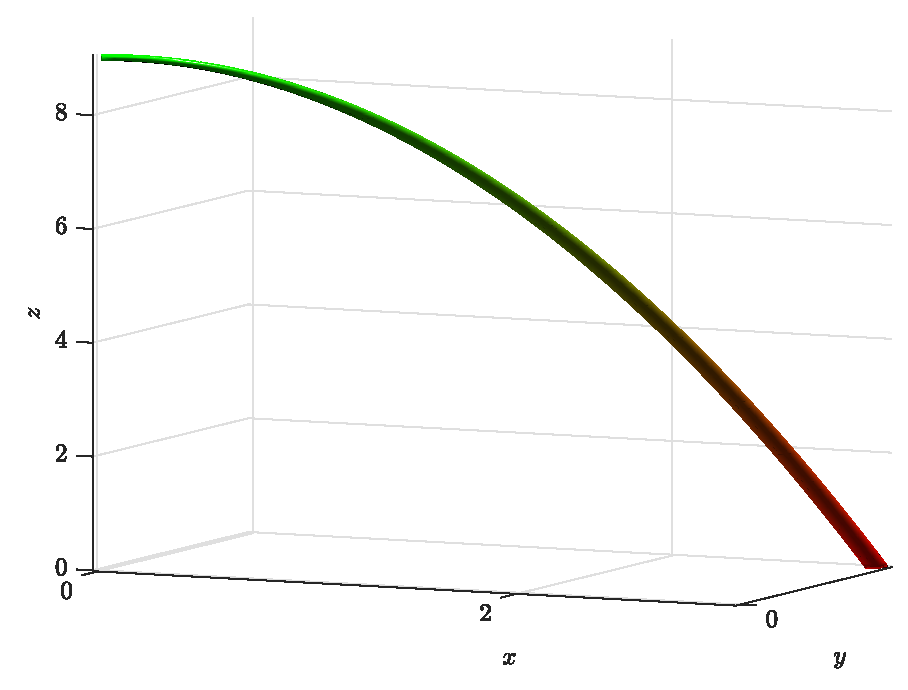
\includegraphics[width=.65\textwidth]{figures/falling_ball}
        \caption{Falling ball. $t=0$ bright green and $t=3$ red.}
    \end{figure}
    \item Here is the plot.
    \begin{figure}[H]
        \centering
        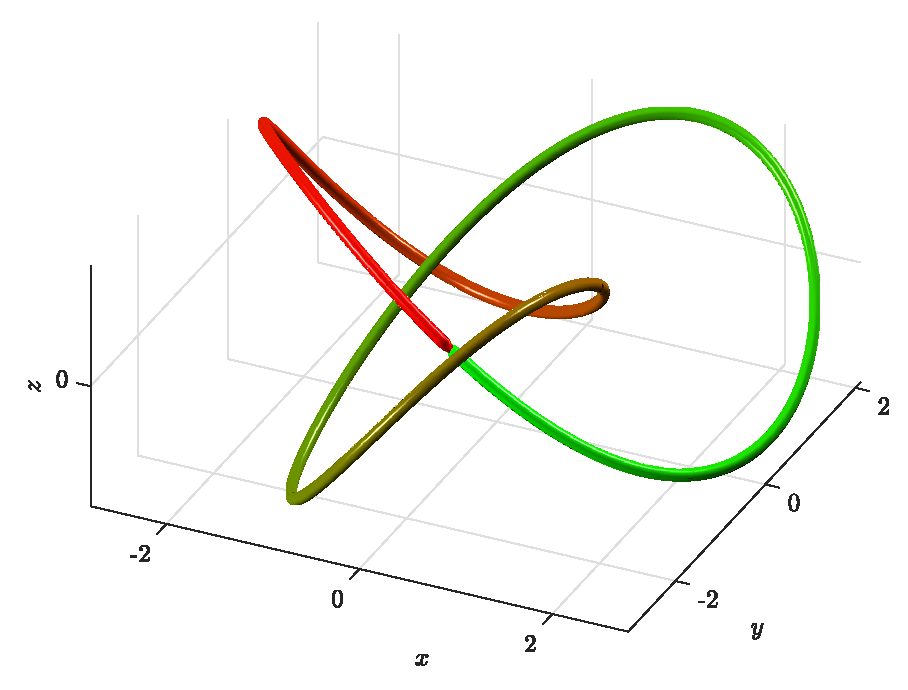
\includegraphics[width=.65\textwidth]{figures/trefoil_knot}
        \caption{Trefoil knot. $t=0$ bright green and $t=2\pi$ red.}
    \end{figure}
\end{enumerate}
\item And an extra plot of my own. Here, I used the equation
\[
\curvegamma = \begin{pmatrix} (5+3\cos(8t))\cos(t) \\ (5+3\cos(8t))\sin(t) \\ 3\sin(8t) \end{pmatrix}
\]
\begin{figure}[H]
    \centering
    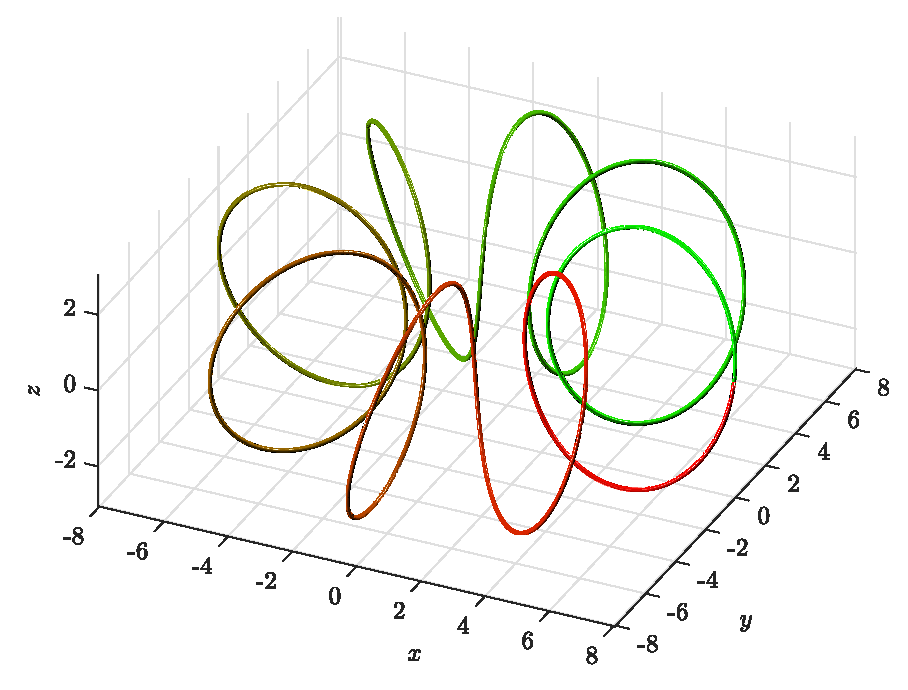
\includegraphics[width=.8\textwidth]{figures/torus_knot}
    \caption{A knot that can be tied around a torus (i.e., the surface of a donut). The trefoil knot is also a torus knot!  $t=0$ bright green and $t=2\pi$ red.}
\end{figure}
\end{solution}


\newpage
\begin{problem}
The length of a curve is an important notion. In fact, the length of a curve is often related to the energy of some configuration. We can compute the length of a curve over the time $t=t_0$ to $t=t_1$ by integrating the \emph{speed} of the curve over that time.  That is,
\[
\ell(\curvegamma) = \int_{t_0}^{t_1} \left|\tangentgamma(t)\right| d t.
\]
We can compute the \emph{energy} of a curve by taking
\[
E(\curvegamma) = \int_{t_0}^{t_1} \frac{1}{2} \left| \tangentgamma(t)\right|^2 d t.
\]
Find the length and energy of the Helix from Problem 1 (a).
\end{problem}

\begin{solution}
We let $\curvegamma(t) = \begin{pmatrix} 3\cos (t) \\ 3\sin(t) \\ t\end{pmatrix}$ and we go from $t=0$ to $t=2\pi$. Then we have
\[
\tangentgamma(t) =\begin{pmatrix} -3\sin(t) \\ 3\cos(t) \\ 1\end{pmatrix}.
\]
and so
\[
\left|\tangentgamma(t)\right| = \sqrt{(-3\sin (t))^2+(3\cos (t))^2+1^2} = \sqrt{10},
\]
since $\sin^2(t)+\cos^2(t)=1$. Now we integrate to find
\begin{align*}
    \ell(\curvegamma) &= \int_0^{2\pi} \sqrt{10}dt\\
    &= \sqrt{10} t|_0^{2\pi}\\
    &= 2\pi \sqrt{10}.
\end{align*}

The energy can be found without too much more work. We have
\[
\left| \tangentgamma(t) \right|^2 = 10,
\]
based on our work before and so
\[
E(\curvegamma) = \int_0^{2\pi} 5 dt = 10 \pi.
\]
\end{solution}

\newpage
\begin{problem}
Given a scalar field of two variables $f(x,y)$, we can create an object called the \emph{graph} of $f(x,y)$ by plotting the set of points $(x,y,f(x,y))$. In fact, you have done this many times in your life. For example, you have consistently plotted the graph of a function $f(x)$ by plotting $(x,f(x))$ in the plane!  

Using GeoGebra, plot the graph of the following functions. Print these off and include them.  Also, describe the what the graph of the function does as we move along the $x$-axis, the $y$-axis, and along the line $y=x$. For each, use the range $-3\leq x \leq 3$ and $-3\leq y \leq 3$.
\begin{enumerate}[(a)]
	\item $f(x,y) = \frac{4xy}{1+x^2+y^2}$.
	\item $g(x,y) = \sin(xy)$.
	\item $h(x,y) = \frac{-x^2-y^2}{5}$.
\end{enumerate}
\end{problem}
\begin{solution}~
\begin{enumerate}[(a)]
    \item Below is the graph of the function $F(x,y)$.
    \begin{figure}[H]
        \centering
        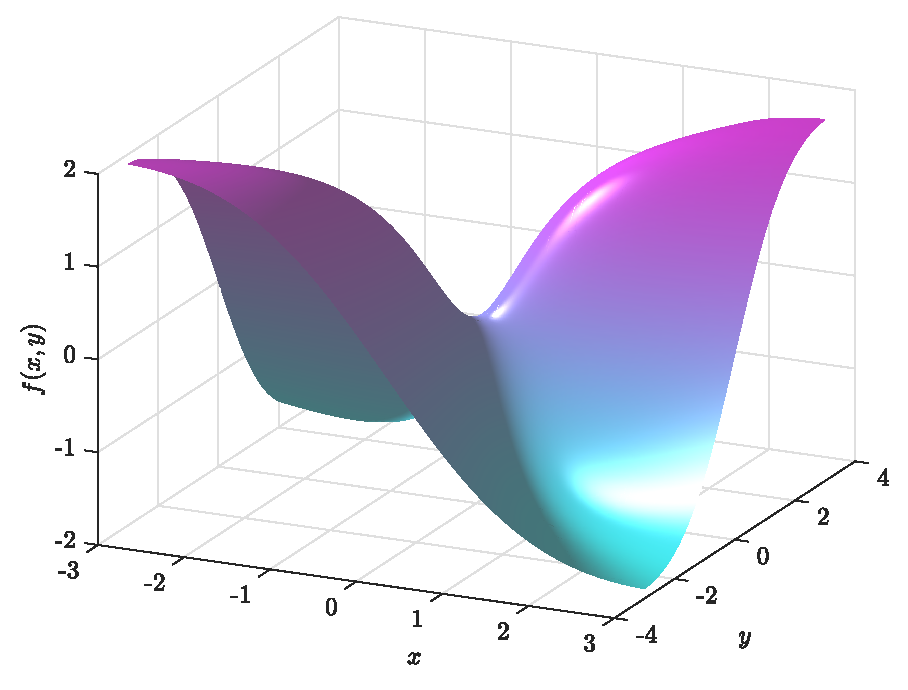
\includegraphics[width=.65\textwidth]{figures/3a}
        \caption{The graph of $f(x,y)$.}
    \end{figure}
    If we move along the $x$-axis, then we have that $y=0$ and thus our function takes the form
    \[
    f(x,0) = \frac{4x\cdot 0}{1+x^2+0^2} = 0.
    \]
    Thus, along this axis the function is a constant zero. Similarly, if we take $x=0$ we have that $F(0,y)=0$ and our function is again constantly zero along this axis. Instead, if we take the function along the $y=x$ line, then we have
    \[
    f(x,x) = \frac{4x^2}{1+2x^2}
    \]
    We can plot this function as a single variable graph in the $(x=y)z$-plane by:
    \begin{figure}[H]
    	\centering
    	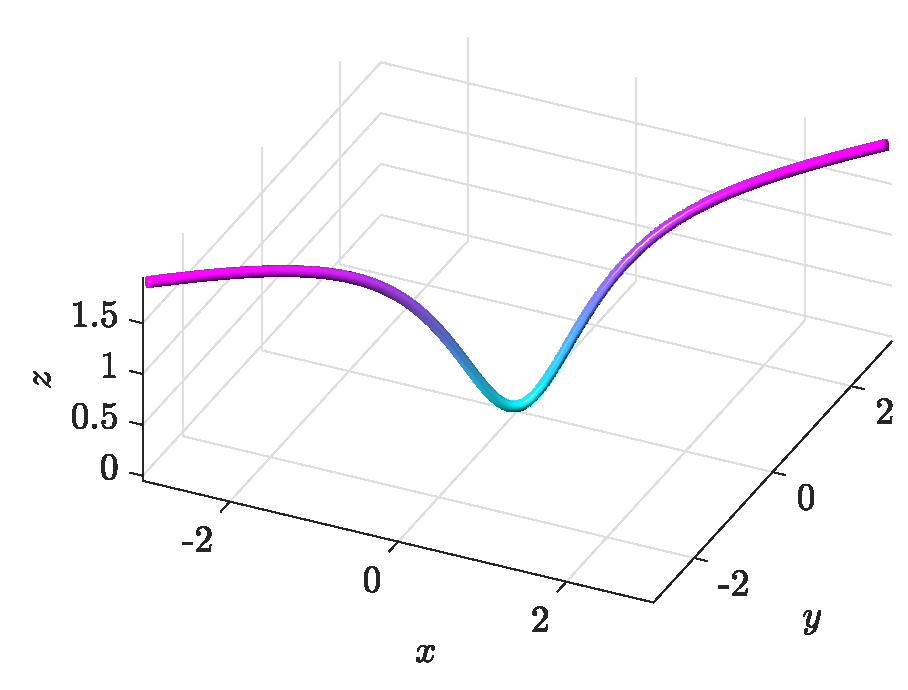
\includegraphics[width=.6\textwidth]{figures/3a_x=y}
    	\caption{The slice of $f(x,y)$ when $x=y$.}
    \end{figure}
    \item Below is the graph of the function $g(x,y)$.
    \begin{figure}[H]
        \centering
        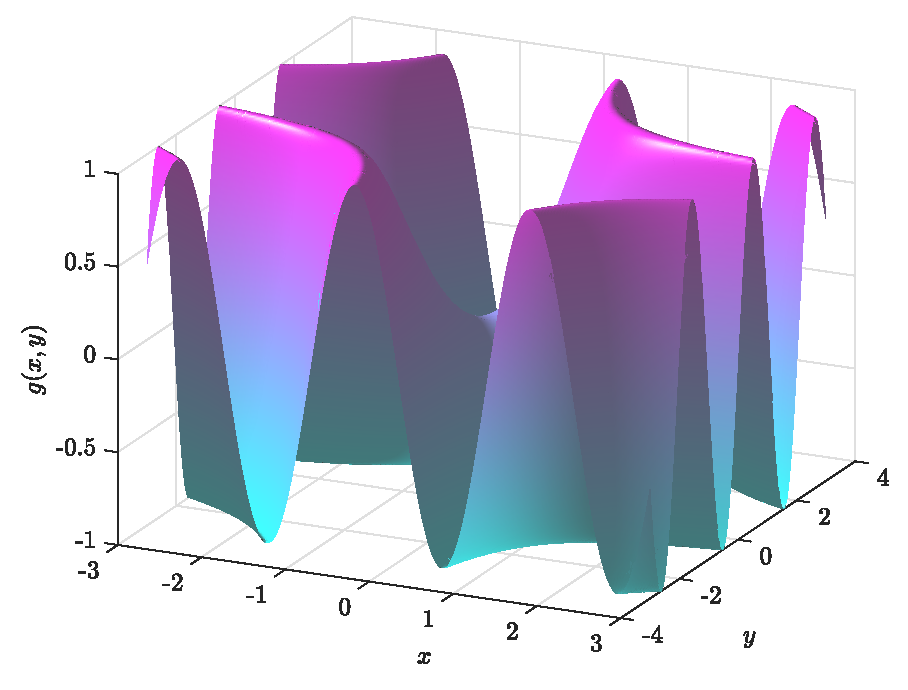
\includegraphics[width=.65\textwidth]{figures/3b}
        \caption{The graph of $g(x,y)$.}
    \end{figure}
    If we move along the $x$-axis, we take $y=0$ and thus
    \[
    g(x,0) = \sin(0) = 0.
    \]
    Hence, our function is constantly zero on this axis.  Similarly, if we take the function on the $y$-axis, then $x=0$ means
    \[
    g(0,y) = 0.
    \]
    Lastly, if we take $y=x$, then
    \[
    g(x,x) = \sin(x^2),
    \]
    which we can graph as a slice.
        \begin{figure}[H]
        	\centering
        	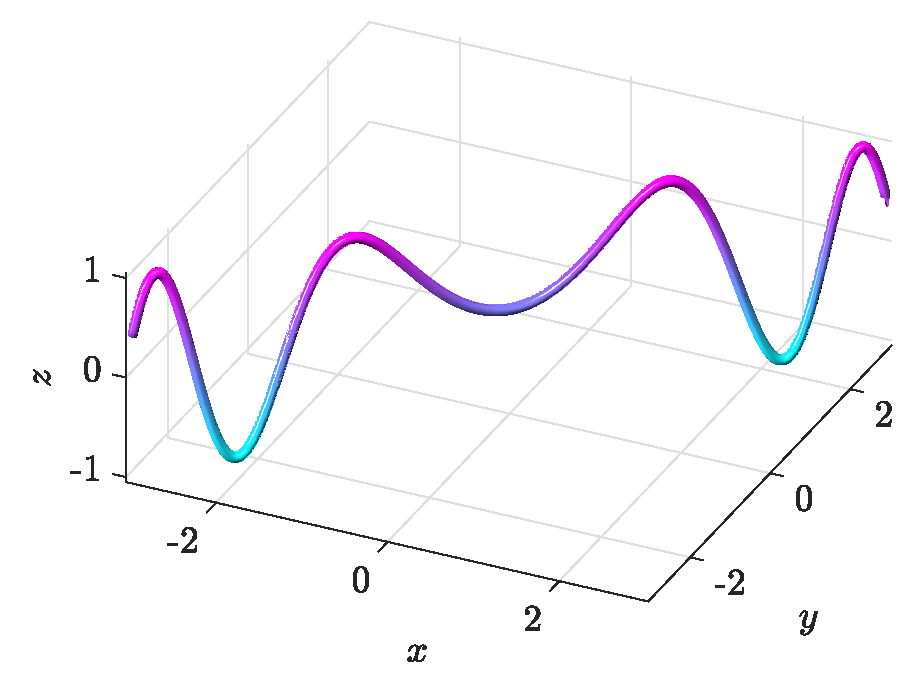
\includegraphics[width=.8\textwidth]{figures/3b_x=y}
        	\caption{The slice of $g(x,y)$ when $x=y$.}
        \end{figure}
    \item Below is the graph of $h(x,y)$.
    \begin{figure}[H]
        \centering
        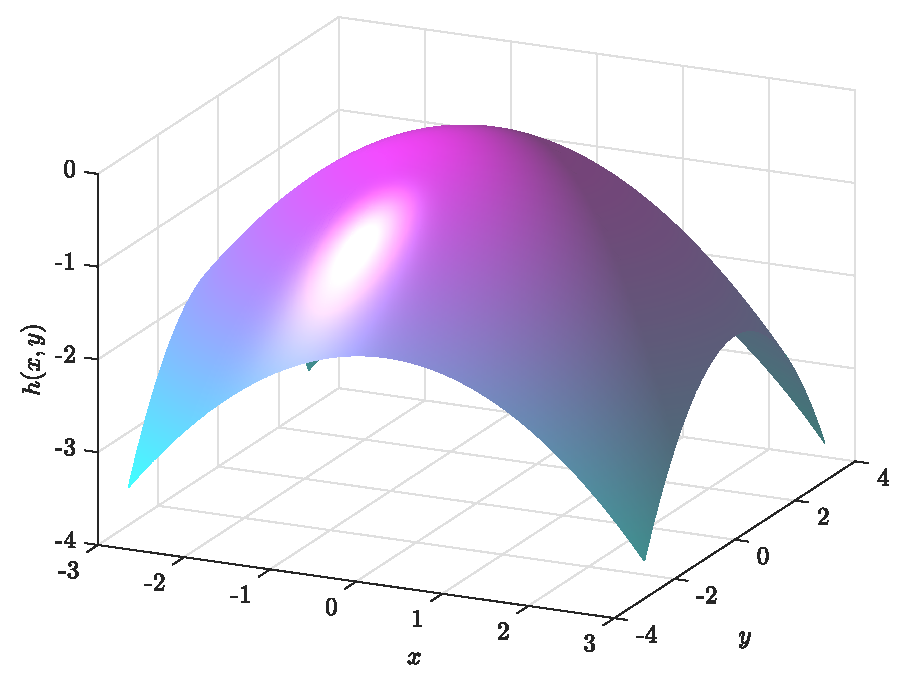
\includegraphics[width=.8\textwidth]{figures/3c}
        \caption{The graph of $h(x,y)$.}
    \end{figure}
    Here if we consider the function along the $x$-axis, we have
    \[
    h(x,0)= \frac{-x^2}{5},
    \]
    which is a parabola in the $xz$-plane. Similarly, on the $y$-axis, we have
    \[
    h(0,y) = \frac{-y^2}{5},
    \]
    which is the same parabola but in the $yz$-plane. Lastly, letting $x=y$ we get
    \[
    h(x,x) = \frac{-2x^2}{5},
    \]
    which also gives us a slice.
        \begin{figure}[H]
        \centering
        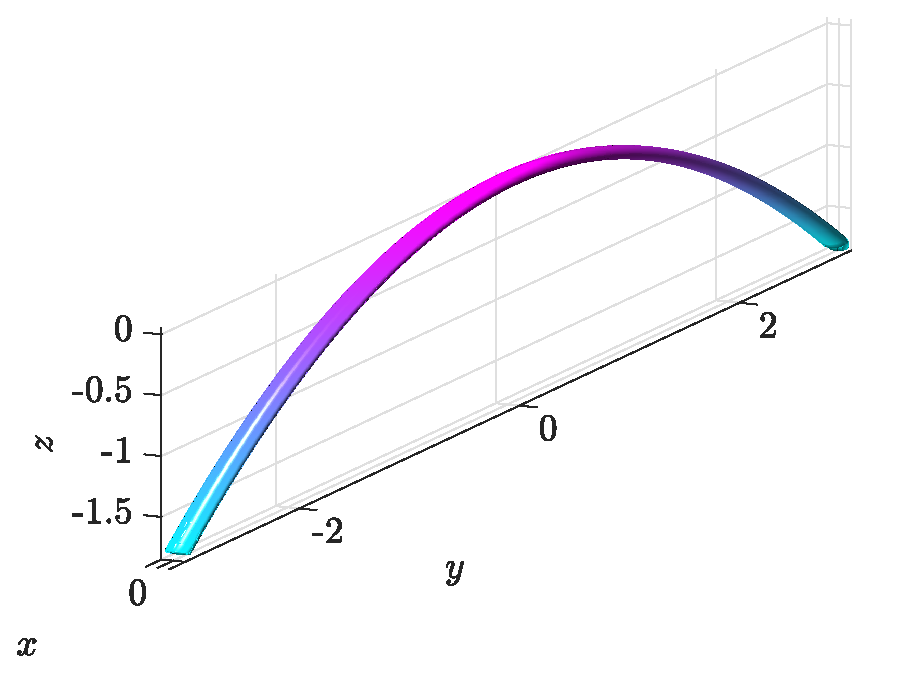
\includegraphics[width=.8\textwidth]{figures/3c_x=0}
        \caption{The slice of $h(x,y)$ when $x=0$.}
    \end{figure}
    \begin{figure}[H]
        \centering
        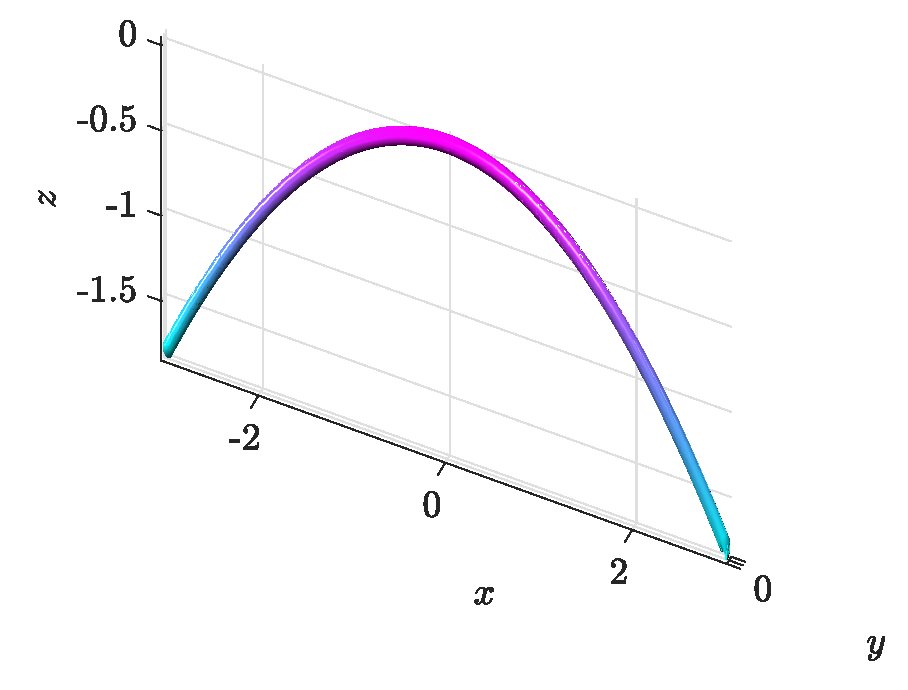
\includegraphics[width=.8\textwidth]{figures/3c_y=0}
        \caption{The slice of $h(x,y)$ when $y=0$.}
    \end{figure}
    \begin{figure}[H]
        \centering
        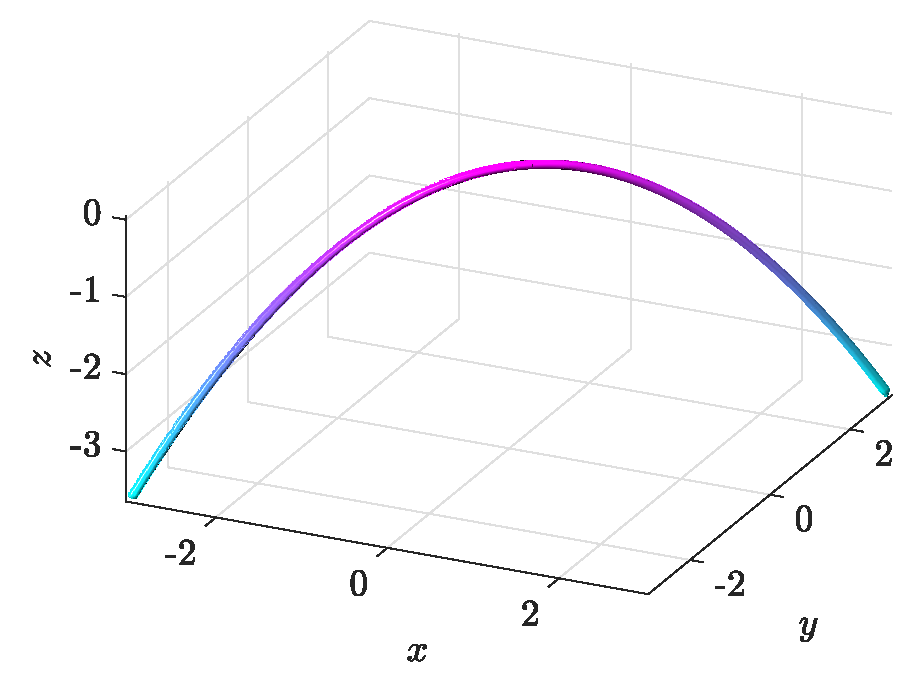
\includegraphics[width=.8\textwidth]{figures/3c_x=y}
        \caption{The slice of $h(x,y)$ when $x=y$.}
    \end{figure}
\end{enumerate}
\end{solution}

\newpage
\begin{problem} 
Let us visualize vector fields using GeoGebra (specifically \url{https://www.geogebra.org/m/u3xregNW}). Plot the following vector fields and print them out. 
\begin{enumerate}[(a)]
    \item (Constant wind from the northwest) $\vecfieldV(x,y)=\begin{pmatrix} 1 \\ -1 \\ 0\end{pmatrix}$.
    \item (Two wind fronts meeting) $\vecfieldU(x,y,z)=\begin{pmatrix} y \\ x \\ 0 \end{pmatrix}$.
    \item (Source) $\vecfieldE(x,y,z) = \begin{pmatrix} \frac{x}{(x^2+y^2+z^2)^{3/2}} \\ \frac{y}{(x^2+y^2+z^2)^{3/2}} \\ \frac{z}{(x^2+y^2+z^2)^{3/2}} \end{pmatrix}$.
    \item (Vortex) $\boldsymbol{\vec{S}}(x,y,z)=\begin{pmatrix} \frac{-y}{x^2+y^2+z^2} \\ \frac{x}{x^2+y^2+z^2} \\ 0\end{pmatrix}.$           
\end{enumerate}
\end{problem}

\begin{solution}~
\begin{enumerate}[(a)]
    \item Here is a plot for $\vecfieldV$.
    \begin{figure}[H]
        \centering
        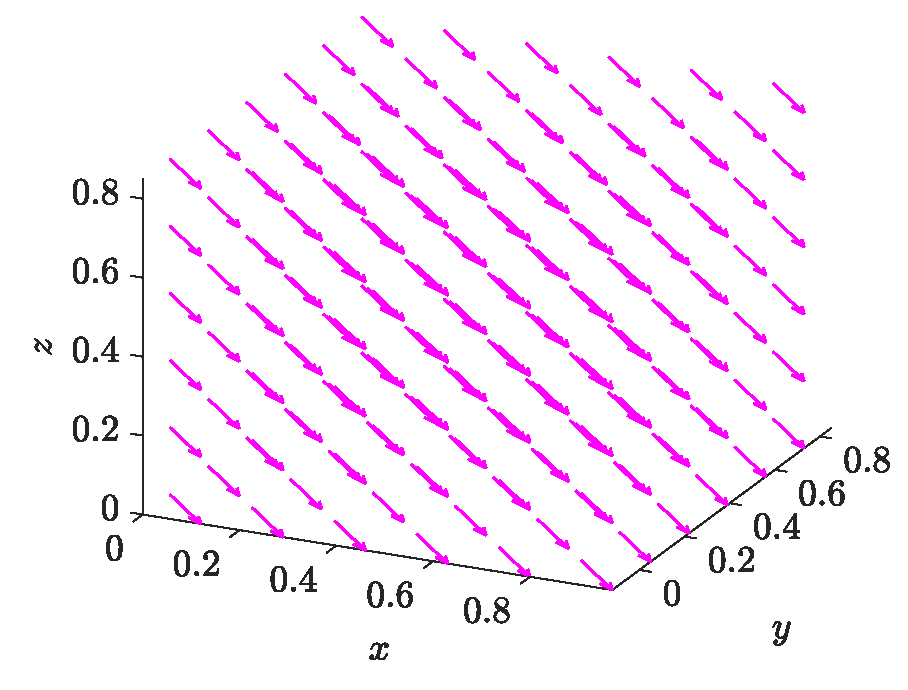
\includegraphics[width=.75\textwidth]{figures/4a}
        \caption{Plot for $\vecfieldV(x,y,z)$.}
    \end{figure}
    \newpage
    \item Here is a plot for $\vecfieldU$.
    \begin{figure}[H]
        \centering
        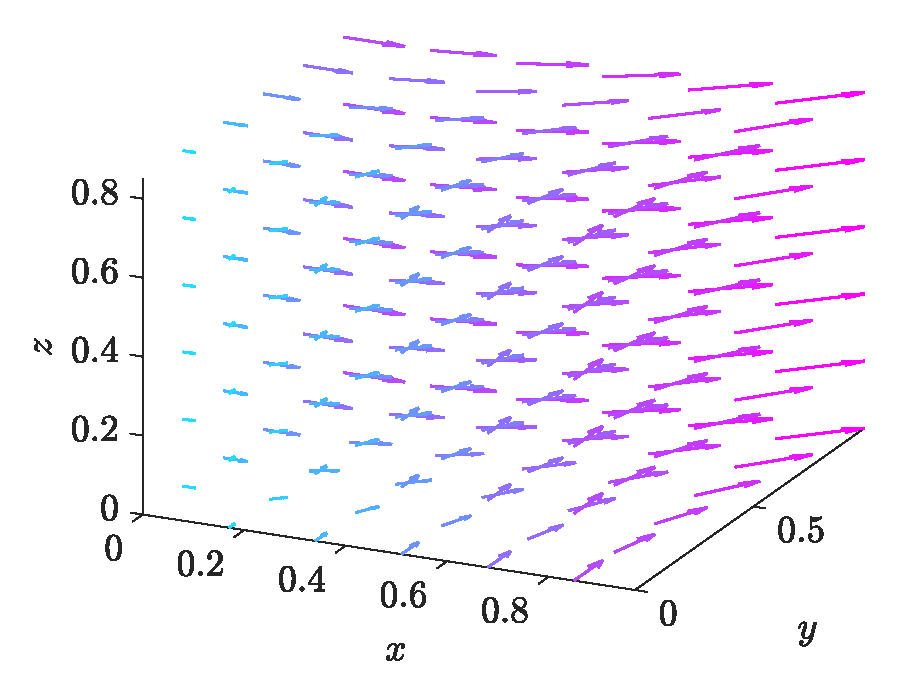
\includegraphics[width=.75\textwidth]{figures/4b}
        \caption{Plot for $\vecfieldU(x,y,z)$.}
    \end{figure}
    \item Here is a plot for $\vecfieldE$.
    \begin{figure}[H]
        \centering
        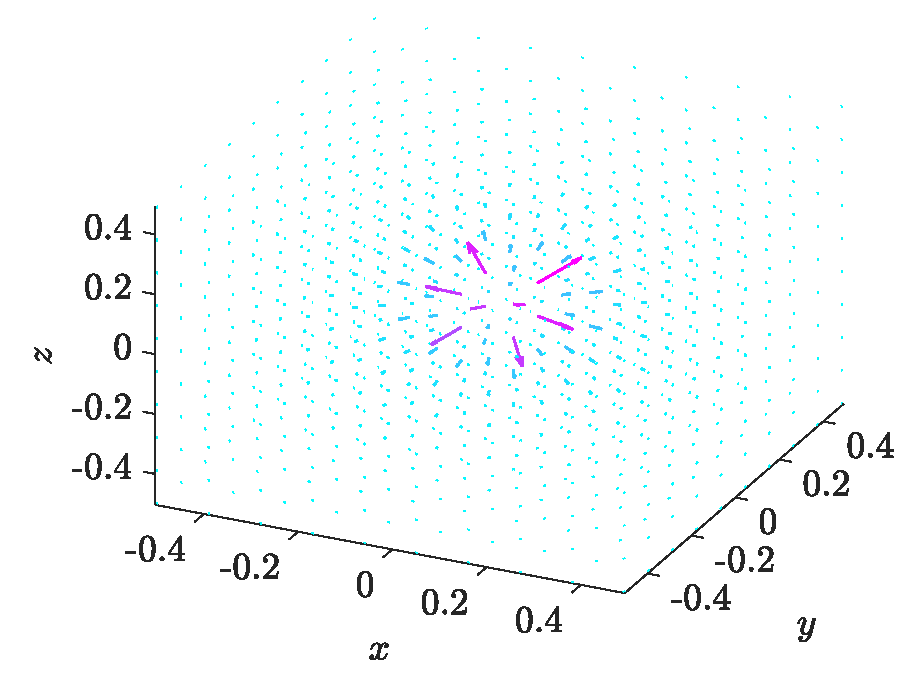
\includegraphics[width=.75\textwidth]{figures/4c}
        \caption{Plot for $\vecfieldE(x,y,z)$.}
    \end{figure}
    \item Here is a plot for $\boldsymbol{\vec{S}}$.
    \begin{figure}[H]
        \centering
        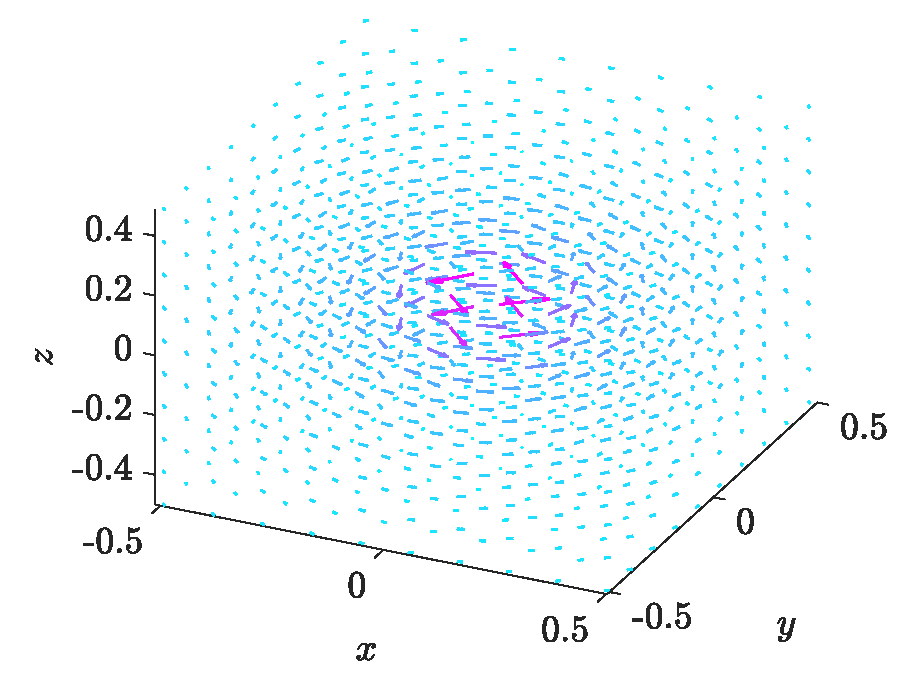
\includegraphics[width=.65\textwidth]{figures/4d}
        \caption{Plot for $\boldsymbol{\vec{S}}(x,y,z)$.}
    \end{figure}
\end{enumerate}
\end{solution}



\newpage
\begin{problem}
Compute the divergence and curl of the Source and Vortex fields from Problem 4 (c) and (d).  What can we say about the divergence and curl of these fields at the origin?
\end{problem}
\begin{solution}
    First, let us take the curl of $\vecfieldE$.  We have
    \begin{align*}
        \grad \times \vecfieldE &= \begin{pmatrix} \frac{\partial E_3}{\partial y} - \frac{\partial E_2}{\partial z} \\ \frac{\partial E_1}{\partial z} -\frac{\partial E_3}{\partial 1} \\ \frac{\partial E_2}{\partial x} - \frac{\partial E_1}{\partial y} \end{pmatrix}\\
        &= \begin{pmatrix} \frac{-3yz}{(x^2+y^2+z^2)^{5/2}} - \frac{-3yz}{(x^2+y^2+z^2)^{5/2}} \\ \frac{-3xz}{(x^2+y^2+z^2)^{5/2}} - \frac{-3xz}{(x^2+y^2+z^2)^{5/2}} \\
        \frac{-3xy}{(x^2+y^2+z^2)^{5/2}} -\frac{-3xy}{(x^2+y^2+z^2)^{5/2}} \end{pmatrix}\\
        &= \begin{pmatrix} 0 \\ 0 \\ 0 \end{pmatrix}.
    \end{align*}
    At the origin, this curl is also identically zero.  The curl of $\vecfieldE$ is simply zero everywhere.
    
    Next, the curl of $\boldsymbol{\vec{S}}$,
        \begin{align*}
            \grad \times \boldsymbol{\vec{S}} &= \begin{pmatrix} 0 - \frac{-2xz}{(x^2+y^2+z^2)^2} \\ \frac{2yz}{(x^2+y^2+z^2)^2} - 0 \\
            \frac{-x^2+y^2+z^2}{(x^2+y^2+z^2)^2}- \frac{x^2-y^2+z^2}{(x^2+y^2+z^2)^2}\end{pmatrix}\\
            &= \begin{pmatrix}  \frac{2xz}{(x^2+y^2+z^2)^2} \\ \frac{2yz}{(x^2+y^2+z^2)^2} \\ \frac{z^2}{(x^2+y^2+z^2)^2}. \end{pmatrix}.
        \end{align*}
    Note that at the origin, we have a discontinuity.  Specifically, the curl at the origin will go to infinity (in each direction) at the origin since the numerator of each component of the curl is of lesser degree (2) than the denominator (4).
    
    The divergence of $\vecfieldE$ is
    \begin{align*}
        \grad \cdot \vecfieldE &= \frac{\partial E_1}{\partial x} + \frac{\partial E_2}{\partial y} + \frac{\partial E_3}{\partial z}\\
        &= \frac{-2x^2+y^2+z^2}{(x^2+y^2+z^2)^{5/2}} + \frac{x^2-2y^2+z^2}{(x^2+y^2+z^2)^{5/2}} + \frac{x^2+y^2-2z^2}{(x^2+y^2+z^2)^{5/2}}\\
        &= 0.
    \end{align*}
    It appears that the divergence of this field $\vecfieldE$ is zero, however this is not actually true at the origin. We will revisit this later, but for now it should be fairly clear that the denominator goes to zero more quickly than the numerator. Indeed, we actually have
    \[
        \grad \cdot \vecfieldE = \delta(\vecx),
    \]
    where $\delta(\vecx)$ is the Dirac delta.
    
    Similarly, the divergence of $\boldsymbol{\vec{S}}$
    \begin{align*}
        \grad \cdot \boldsymbol{\vec{S}} &= \frac{2xy}{(x^2+y^2+z^2)^2} + \frac{-2xy}{(x^2+y^2+z^2)^2}\\
        &=0.
    \end{align*}
    Once again, this appears to be zero everywhere (including the origin). But one should be weary of whether or not this is totally true!
\end{solution}


\begin{problem}
Consider the following scalar field and vector field
\[
f(x,y,z) = x^2+y^2-z^2 \qquad \textrm{and} \qquad \vecfieldV(x,y,z) = \begin{pmatrix} -y \\ x \\ z \end{pmatrix}.
\]
\begin{enumerate}[(a)]
    \item Compute all first order partial derivatives of $f$.
    \item Show that $\frac{d^2 f}{d x d y} = \frac{d^2 f}{d y d x}$.
    \item Explain why $\vecfieldV$ has nonzero curl when $x$ and $y$ are nonzero using a physical argument. (\emph{Hint: What plane would a rod start rotating in?})
    \item Explain why $\vecfieldV$ has nonzero divergence when $z\neq 0$ using a physical argument. (\emph{Hint: In what direction would a particle start accelerating towards infinity?})
    \item Compute the directional derivative of $f$ at $\vecx_0 = (1,2,-3)$ in the direction of $\vecfieldV(\vecx_0)$.
\end{enumerate}
\end{problem}
\begin{solution}
\begin{enumerate}[(a)]
    \item We have
    \begin{align*}
        \frac{\partial f}{\partial x} &= 2x, \\
        \frac{\partial f}{\partial y} &= 2y, \\
        \frac{\partial f}{\partial z} &= -2z.
    \end{align*}
    \item Taking the next derivatives we get
    \[
        \frac{\partial }{\partial x} \frac{\partial f}{\partial y} = 2
    \]
    and
    \[
        \frac{\partial}{\partial y}\frac{\partial f}{\partial x} = 2,
    \]
    and so $\frac{d^2 f}{d x d y} = \frac{d^2 f}{d y d x}$.

    \item First, here is a generic view of the vector field $\vecfieldV$.
        \begin{figure}[H]
        \centering
        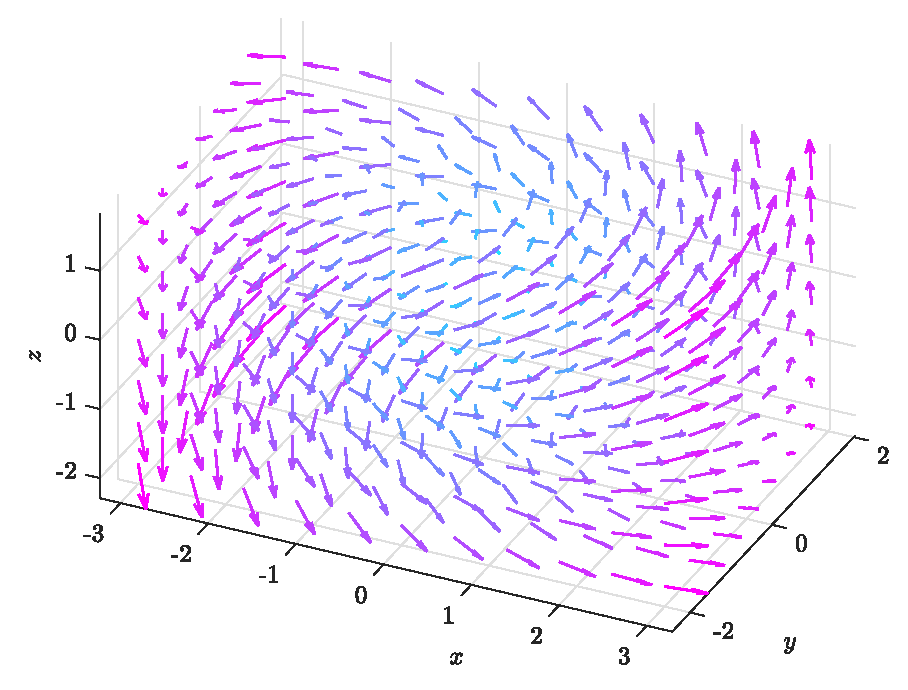
\includegraphics[width=.65\textwidth]{figures/6c_field}
    \end{figure}
        Let's examine the vector field $\vecfieldV$ by looking down at the $xy$-plane. When we do this, we see the following.
        \begin{figure}[H]
        \centering
        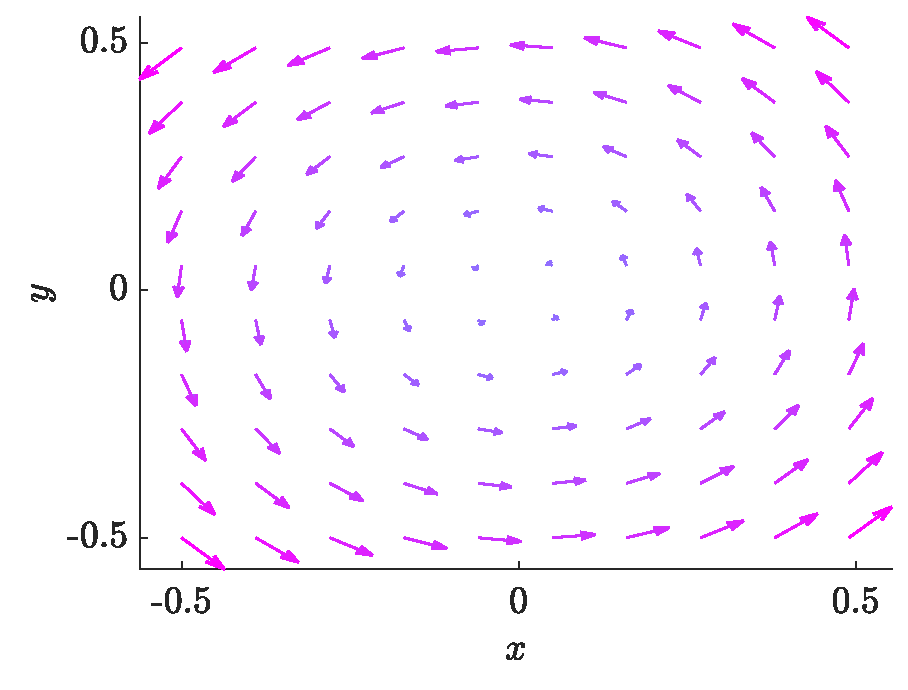
\includegraphics[width=.65\textwidth]{figures/6c}
        \caption{Plot looking down at the $xy$-plane shows circular motion.}
    \end{figure}
    Since we see vectors that would torque a rod parallel with the $xy$-plane we that for any value of $z$ there is curl. However a particle at $x=0$ and $y=0$ will not move at all.

    \item Next, take a look at $\vecfieldV$ while aligning the $z$-axis vertically to see the following picture.
        \begin{figure}[H]
        \centering
        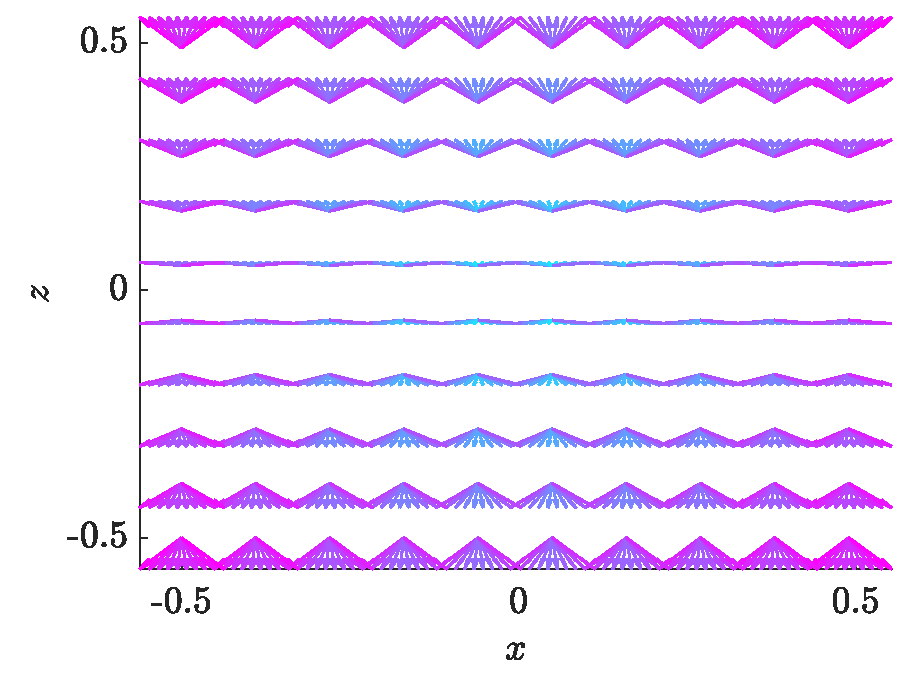
\includegraphics[width=.65\textwidth]{figures/6d}
        \caption{Plot looking down at the $xy$-plane shows circular motion.}
    \end{figure}
    If we place any particle with $z\neq 0$ then the particle will accelerate away from the $xy$-plane.
\end{enumerate}

    \item To compute this directional derivative, we need to compute a few items. First, we have the gradient
    \[
        \grad f = \begin{pmatrix} 2x \\ 2y \\ -2z \end{pmatrix}.
    \]
    Next, we evaluate both $\grad f$ and $\vecfieldV$ at $\vecx_0$
    \[
    \grad f(\vecx_0) = \begin{pmatrix} 2 \\ 4 \\ 6 \end{pmatrix} \qquad \textrm{and} \qquad \vecfieldV(\vecx_0) = \begin{pmatrix} -2 \\ 1 \\ -3 \end{pmatrix}.
    \]
    Now, we need a unit vector pointing in the same direction as $\vecfieldV(\vecx_0)$ so we have
    \[
    \unitvec = \frac{1}{|\vecfieldV(\vecx_0)|} \vecfieldV(\vecx_0) = \frac{1}{\sqrt{14}} \begin{pmatrix} -2 \\ 1 \\ -3 \end{pmatrix}.
    \]
    Then, the intended directional derivative is
    \[
    \boxed{\unitvec\cdot \grad f(\vecx_0) = \frac{1}{\sqrt{14}} \begin{pmatrix} -2 \\ 1 \\ -3 \end{pmatrix} \cdot \begin{pmatrix} 2 \\ 4 \\ 6 \end{pmatrix} = \frac{-18}{\sqrt{14}}.}
    \]
\end{solution}

\newpage
\begin{problem}
For this problem, let us consider a family of scalar fields of varying dimensionality. In the previous problem, we plotted the graph of a scalar field with two inputs, but when there are more than two inputs we must resort to other methods of visualization.

In particular, we will seek out an understanding of the \emph{level sets} and how to relate these to the gradient of a scalar field. For each part, compute the set of points such that $f(\vecx)=\frac{1}{2}$, $f(\vecx)=1$, $f(\vecx)=2$, and $f(\vecx)=3$ and plot these sets (including all the different level sets in one plot per function). 

Then for each field, compute the gradient (row) vector
\[
\nablavec f(\vecx) = \begin{pmatrix} \frac{\partial f}{\partial x_1} & \frac{\partial f}{\partial x_2} & \cdots & \frac{\partial f}{\partial x_n}\end{pmatrix}.
\]
Finally, draw an approximation of the the gradient vector field on your plots at a three different points for each part. (\emph{Hint: think of how the gradient relates to level sets of functions!})
\begin{enumerate}[(a)]
	\item Consider the 1-dimensional scalar field 
	\[
	f(x) = |x| = \sqrt{x^2}.
	\]
	Here each level set will be made up of distinct points.
	\item Consider the 2-dimensional scalar field
	\[
	f(x,y) = |\vecx| = \sqrt{x^2+y^2}.
	\]
	Here each level set will be a curve.
	\item Consider the 3-dimensional scalar field
		\[
		f(x,y,z) = |\vecx| = \sqrt{x^2+y^2+z^2}.
		\]
		Here each level set will be a surface.
\end{enumerate}
\end{problem}

\begin{solution}~
\begin{enumerate}[(a)]
    \item We first solve this problem algebraically then we'll deal with the plots.  We have
    \begin{align*}
        f(x)&=c\\
        \iff x^2 &= c^2\\
        \iff x^2&= c^2\\
        \iff x &= -\pm c.
    \end{align*}
    Now using this, we find that the level points follow:
    \begin{align*}
        \textrm{For $c_1=1$:~}\quad x&=\pm 1\\
        \textrm{For $c_2=2$:~}\quad x&=\pm 2\\
        \textrm{For $c_3=3$:~}\quad x&=\pm 2.\\
    \end{align*}
    Here are the plots.
    \begin{figure}[H]
        \centering
        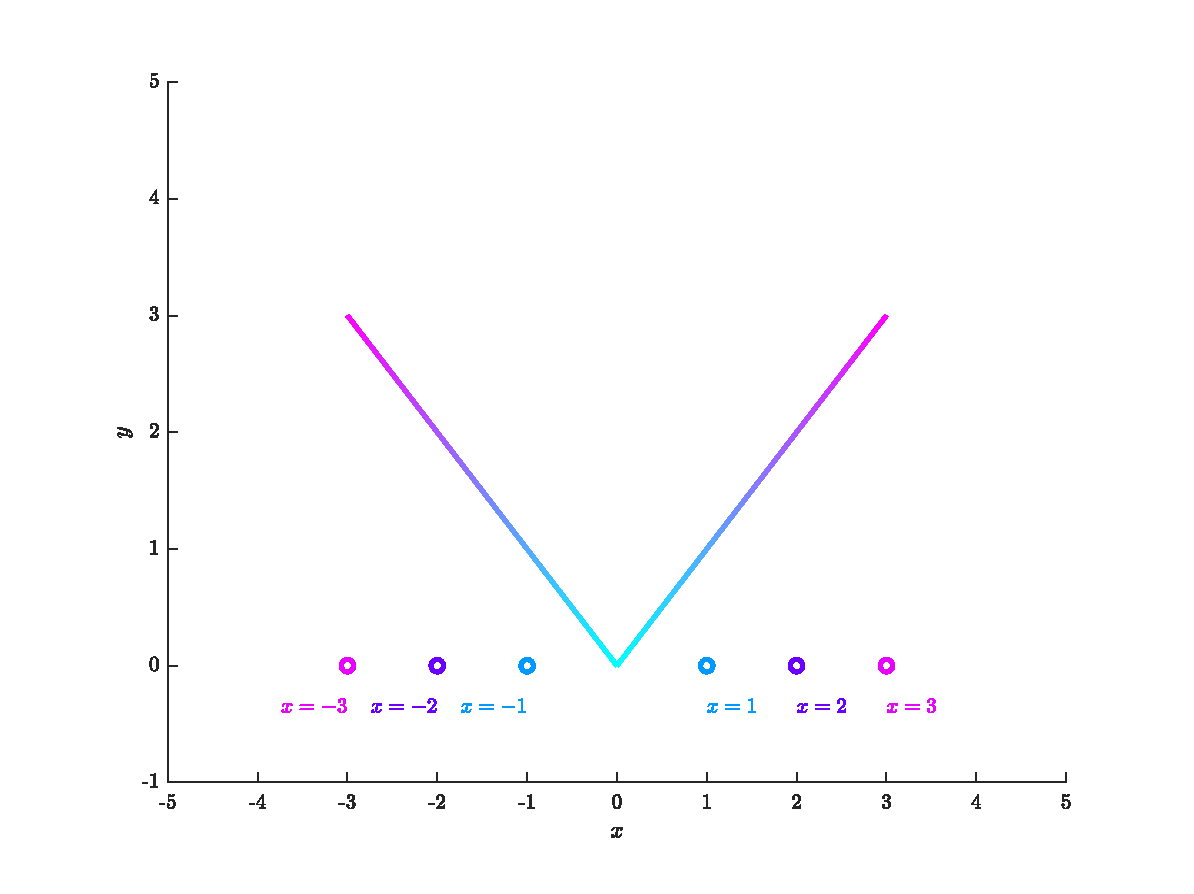
\includegraphics[width=.6\textwidth]{figures/7a}
        \caption{Graph of $f(x)$ with level points on the $x$-axis.}
    \end{figure}
    
    The gradient is then
    \[
    \xhat \frac{\partial}{\partial x} \sqrt{x^2} = \frac{x}{\sqrt{x^2}} = \textrm{sign}(x).
    \]
    The gradient here is either $+1$ when $x>0$ or $-1$ when $x<0$ and it does not exist at $x=0$ as seen in the graph.

    \item Let's repeat the same process as in (a). We take
    \begin{align*}
        f(x,y)&=c\\
        \iff \sqrt{x^2+y^2}&= c\\
        \iff x^2+y^2&=c^2,\\
    \end{align*}
    which is the equation for a circle of radius $c$. Now using this, we find that the level curves follow:
    \begin{align*}
        \textrm{For $c_1=1$:~}\quad x^2+y^2&=1\\
        \textrm{For $c_2=2$:~}\quad x^2+y^2&=2\\
        \textrm{For $c_3=3$:~}\quad x^2+y^2&=3.\\
    \end{align*}
    Here are the plots.
    \begin{figure}[H]
        \centering
        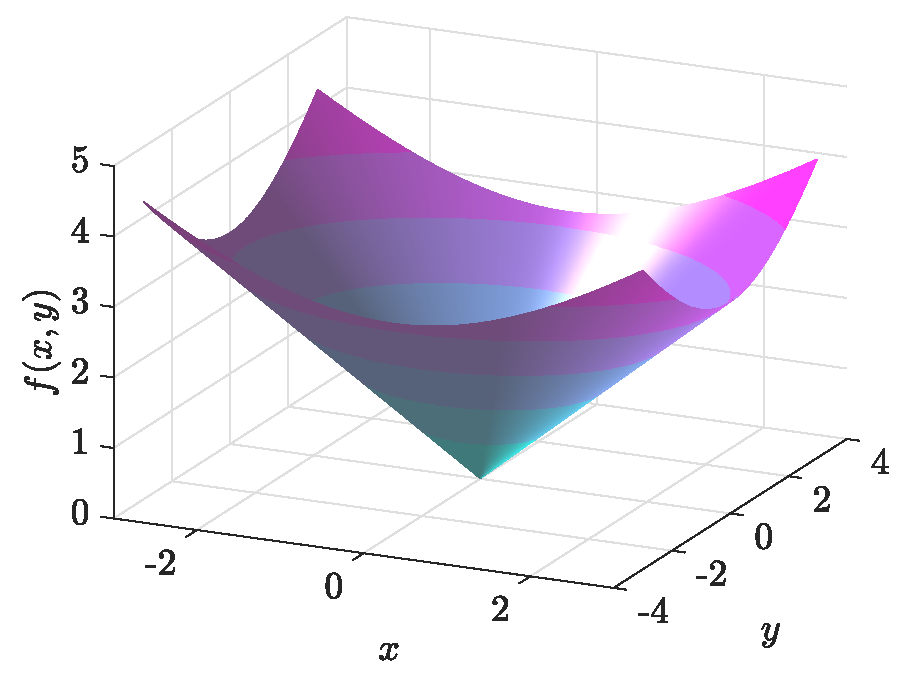
\includegraphics[width=.65\textwidth]{figures/7b_surface}
        \caption{The graph of the function $f(x,y)$.}
    \end{figure}
    \begin{figure}[H]
        \centering
        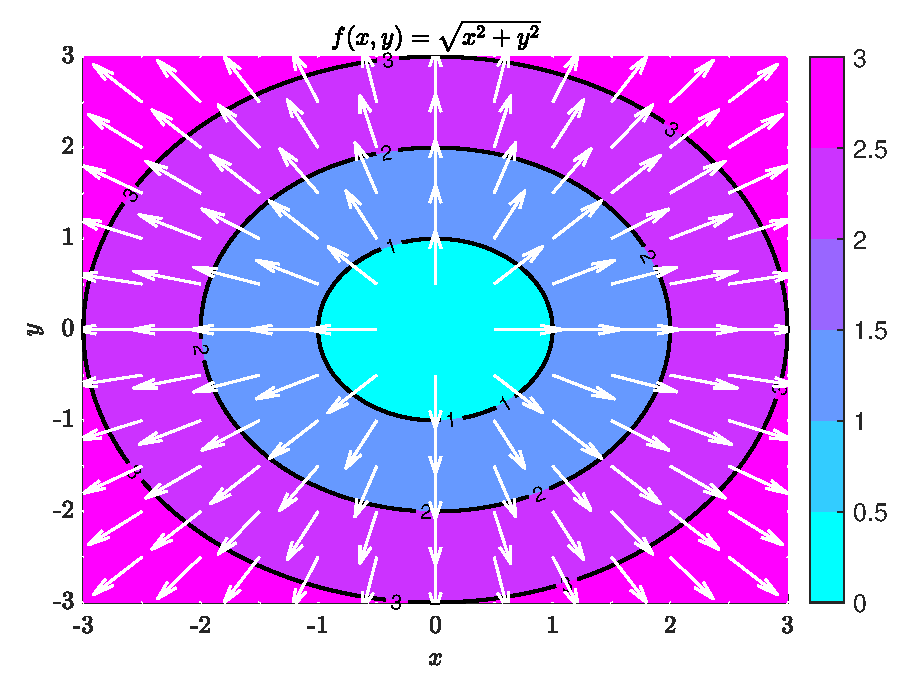
\includegraphics[width=.65\textwidth]{figures/7b_contour}
        \caption{The level curves for the function $f(x,y)$ along with the gradient vector field $\grad f$.}
    \end{figure}
    
    The gradient is
    \[
    \grad f(x,y) = \begin{pmatrix} \frac{x}{\sqrt{x^2+y^2}} \\ \frac{y}{\sqrt{x^2+y^2}} \end{pmatrix},
    \]
    and this is shown in the above figure.

    \item Let's repeat the process one last time, so we have
    \begin{align*}
            f(x,y,z)&=c\\
        \iff \sqrt{x^2+y^2+z^2}&= c,\\
        \iff x^2+y^2+z^2 &= c^2,
    \end{align*}
    which is the equation for a sphere of radius $\frac{1}{c}$.  Then the level surfaces follow:
        \begin{align*}
        \textrm{For $c_1=1$:~}\quad x^2+y^2+z^2&=1\\
        \textrm{For $c_2=2$:~}\quad x^2+y^2+z^2&=2\\
        \textrm{For $c_3=3$:~}\quad x^2+y^2+z^2&=3.\\
    \end{align*}
    Here are the plots
    \begin{figure}[H]
        \centering
        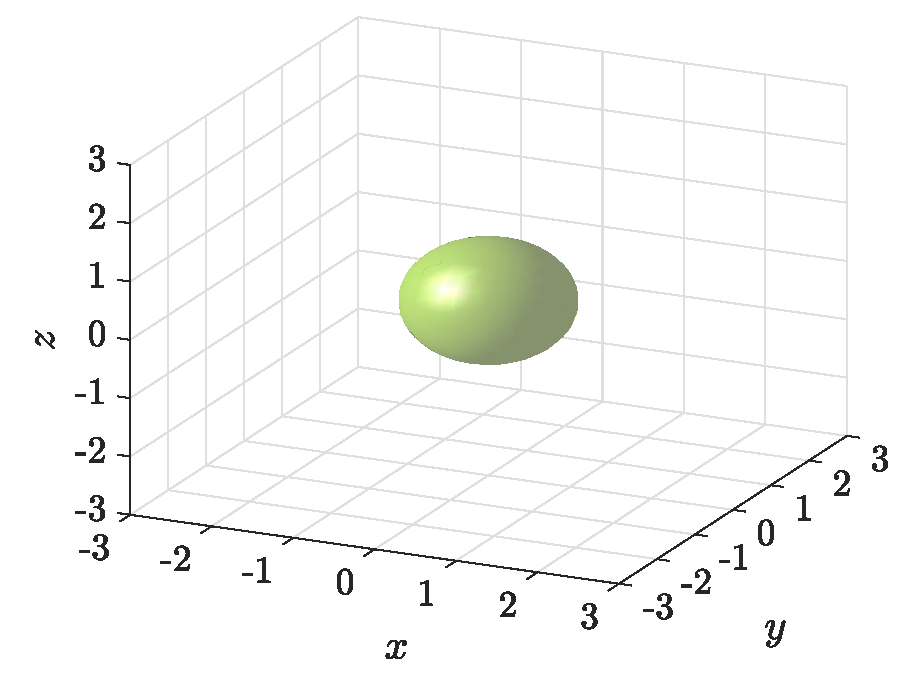
\includegraphics[width=.65\textwidth]{figures/7c_1}
        \caption{Level surface for $f(x,y,z)=1$.}
    \end{figure}
    \begin{figure}[H]
        \centering
        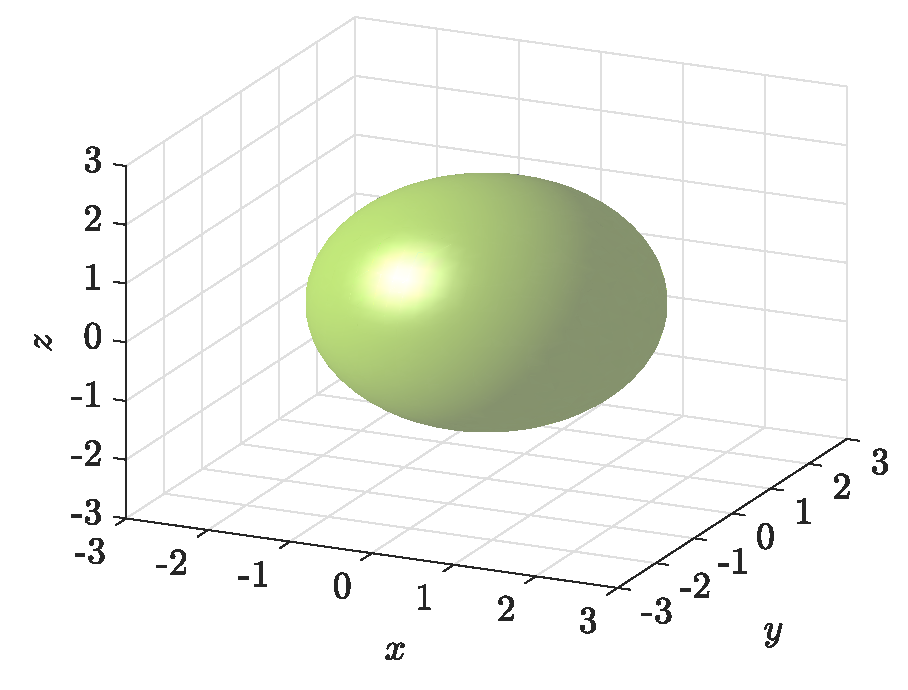
\includegraphics[width=.65\textwidth]{figures/7c_2}
        \caption{Level surface for $f(x,y,z)=2$.}
    \end{figure}
    \begin{figure}[H]
        \centering
        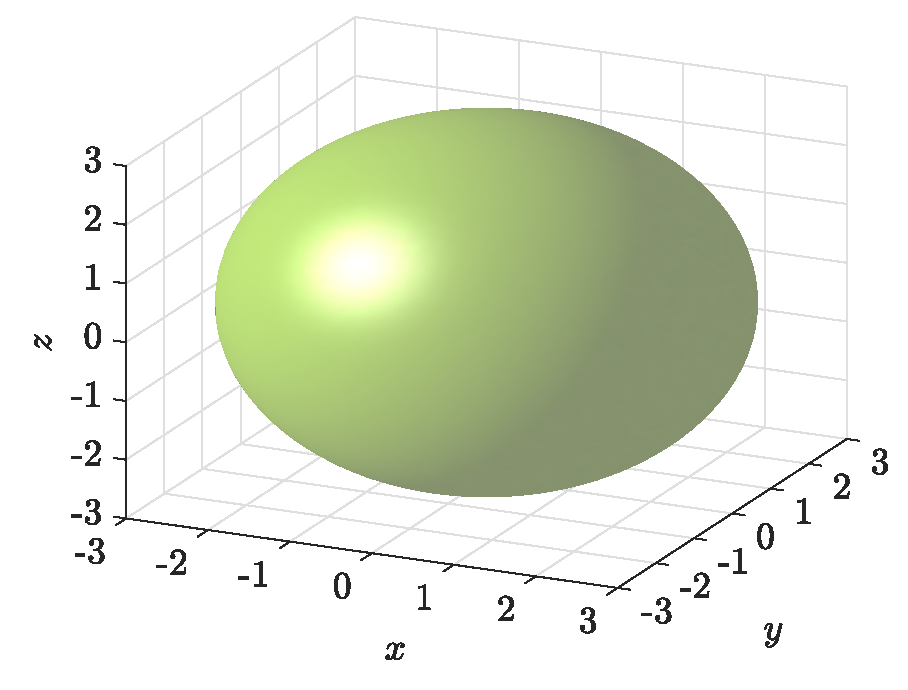
\includegraphics[width=.65\textwidth]{figures/7c_3}
        \caption{Level surface for $f(x,y,z)=3$.}
    \end{figure}

    Finally, we have the gradient
    \[
    \grad f(x,y,z) = \begin{pmatrix} \frac{x}{\sqrt{x^2+y^2+z^2}} \\ \frac{y}{\sqrt{x^2+y^2+z^2}} \\ \frac{z}{\sqrt{x^2+y^2+z^2}} \end{pmatrix}
    \]
    which I plot below.

    \begin{figure}[H]
        \centering
        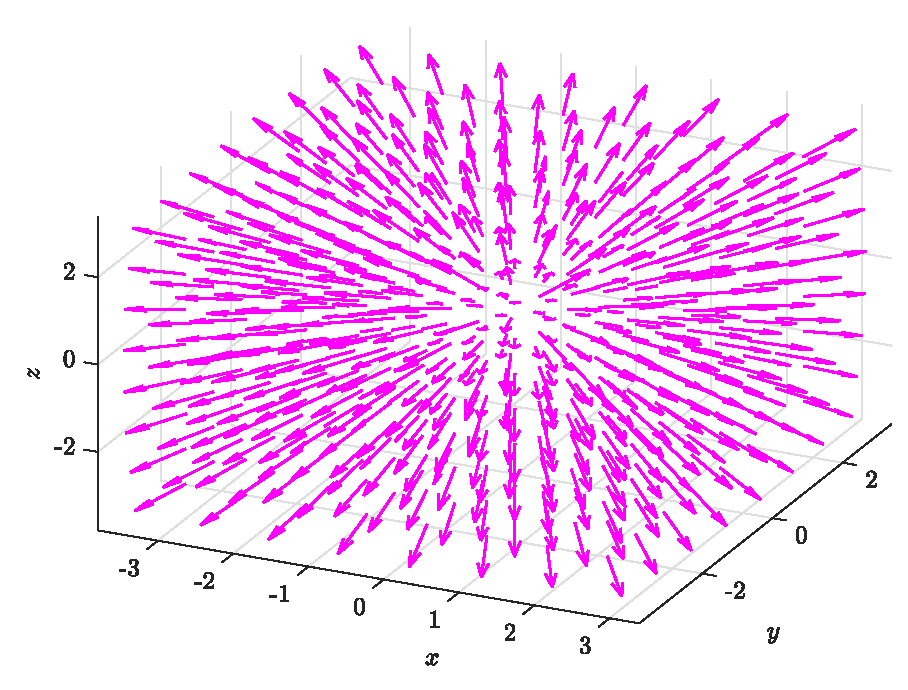
\includegraphics[width=.65\textwidth]{figures/7c_gradient}
        \caption{$\grad f(x,y,z)$.}
    \end{figure}
\end{enumerate}
One can think of these level sets as the sets of constant energy. For example, if this function $f(x,y,z)$ describes the potential energy (which this function does for the gravitational and electrostatic force), then the level sets correspond to the circular orbits of particles in this potential field. 
\end{solution}

%\newpage
%\begin{problem}
%Consider the two dimensional scalar field $T(x,y)=x+y$ that describes the temperature on the square plate $\Omega$ given by the set $0\leq x,y \leq 1$.  Compare the two answers you get!
%\begin{enumerate}[(a)]
%	\item Compute the integral
%	\[
%	\int_\Omega T(x,y)d\Omega.
%	\]
%	\item Let $\curvegamma$ be the curve that traverses the boundary of the square plate in the counterclockwise direction.  Compute
%	\[
%	\int_{\curvegamma} T(\curvegamma)d\curvegamma. 
%	\]
%\end{enumerate}
%\end{problem}
%\begin{solution} ~
%	\begin{enumerate}[(a)]
%		\item We take
%		\begin{align*}
%			\iint_\Omega T(x,y)d\Omega &= \int_0^1 \int_0^1 x+y dxdy\\
%			&= \int_0^1 \left.\left(\frac{1}{2}x^2+xy\right)\right\vert_0^1 dy\\
%			&= \int_0^1 \frac{1}{2} + y dy\\
%			&= \left.\left(\frac{1}{2}y + \frac{1}{2}y^2\right)\right\vert_0^1\\
%			&= 1.
%		\end{align*}
%		\item	First, note that there are four straight curves that parameterize the boundary of the plate.  Namely, we can choose the parameterizations 
%		\[
%		\curvegamma_1(t) = \begin{pmatrix} t \\ 0 \end{pmatrix} \quad \curvegamma_2(t) = \begin{pmatrix} 1 \\ t \end{pmatrix} \quad \curvegamma_1(t) = \begin{pmatrix} 1-t \\ 1 \end{pmatrix} \quad \curvegamma_1(t) = \begin{pmatrix} 0 \\ 1-t \end{pmatrix},
%		\]
%		Note that there are many other parameterizations that work. We can see the chosen curves in this figure:
%		\begin{figure}[H]
%			\centering
%			\includegraphics[width=.6\textwidth]{Images/plate_boundary.png}
%		\end{figure}
%		Thus, our integral can be written as
%		\[
%		\int_{\curvegamma} T(\curvegamma) d\curvegamma = \int_{\curvegamma_1} T(\curvegamma) d\curvegamma_1 + \int_{\curvegamma_2} T(\curvegamma) d\curvegamma_2 + \int_{\curvegamma_3} T(\curvegamma) d\curvegamma_3 + \int_{\curvegamma_4} T(\curvegamma) d\curvegamma_4.
%		\]
%		Then, we can compute each integral on the right hand side.
%		\begin{align*}
%			\int_{\curvegamma_1} T(\curvegamma_1) d\curvegamma_1 &= \int_0^1 T(\curvegamma_1(t))\left|\tangentgamma_1(t)\right|dt\\
%			&= \int_0^1 T(t,0) dt\\
%			&= \int_0^1 t dt\\
%			&= 1.
%		\end{align*}
%		Similarly, 
%		\begin{align*}
%				\int_{\curvegamma_2} T(\curvegamma_2) d\curvegamma_2 &= \int_0^1 T(\curvegamma_2(t))\left|\tangentgamma_2(t)\right|dt\\
%				&= \int_0^1 T(1,t) dt\\
%				&= \int_0^1 1+t dt\\
%				&= \left.\left(t+\frac{1}{2}t^2\right)\right\vert_0^1\\
%				&= \frac{3}{2}.
%		\end{align*}	
%		Again,
%		\begin{align*}
%				\int_{\curvegamma_3} T(\curvegamma_3) d\curvegamma_3 &= \int_0^1 T(\curvegamma_3(t))\left|\tangentgamma_3(t)\right|dt\\
%				&= \int_0^1 T(1-t,1) dt\\
%				&= \int_0^1 (1-t)+1 dt\\
%				&= \int_0^1 2-tdt\\
%				&= \left.\left( 2t-\frac{1}{2}t^2\right)\right\vert_0^1\\
%				&= \frac{3}{2}.
%		\end{align*}			
%		Lastly,
%		\begin{align*}
%			\int_{\curvegamma_4} T(\curvegamma_4) d\curvegamma_4 &= \int_0^1 T(\curvegamma_4(t))\left|\tangentgamma_4(t)\right|dt\\
%			&= \int_0^1 T(0,1-t) dt\\
%			&= \int_0^1 1-t dt\\
%			&= \left.\left(t-\frac{1}{2}t^2\right)\right\vert_0^1\\
%			&= \frac{1}{2}.
%		\end{align*}	
%	\end{enumerate}
%	Thus, we have
%	\[
%	\boxed{\int_{\curvegamma} T(\curvegamma) d\curvegamma = 1+\frac{3}{2}+\frac{3}{2}+\frac{1}{2} = \frac{9}{2}.}
%	\]
%\end{solution}
\end{document}